\begin{abstract}
In this paper, we introduce a general approach to diagnosing
program errors detected by type systems or other program analyses.
This approach works on any analysis that can be described as a
constraint system, in which a detected error corresponds to one or
more unsatisfiable constraints.  Both satisfiable and unsatisfiable
paths through the constraint system are analyzed, to identify the
program expressions most likely to be the cause of the unsatisfiable
constraints. The likelihood of different error explanations is
evaluated under the assumption that the programmer's code is mostly
correct, so the simplest error explanations are chosen, according to
maximum a posteriori principles. For analyses that depend on
programmer-stated assumptions about the environment, the error
diagnosis also identifies likely missing assumptions.  The new error
diagnosis approach has been implemented for two very different program
analyses: type inference in OCaml and information flow checking in
Jif. The effectiveness of the approach is evaluated using a corpus of
previously collected programs containing errors. The results show that
the technique identifies the location of program errors significantly
more accurately than in the original compilers, and also identifies
missing assumptions effectively.

\end{abstract}

\section{Introduction}

Over the past couple of decades, many sophisticated type systems and,
more generally, program analyses have been developed, allowing
complex, important properties of software to be verified. Advances in
type inference, dataflow analysis, and constraint solving have made
programming with such verification more practical, by lowering the
annotation burden and making verification time more acceptable.  Use
of these techniques has become more common, but expressive type
systems are still infrequently used.

We posit that a key barrier to adoption of these sophisticated
analyses is the difficulty of debugging programs when the analysis
reports an error. Because deep, non-local software properties are
being checked, the analysis may detect an inconsistency in a part of
the program that is far from the actual error. Reporting on the
inconsistency at the point of detection can result in a misleading
error message. Determinining where the true error lies based on this
error message can require excessive effort from the programmer, and an
unreasonably high degree of understanding of how the analysis works
in order to interpret the error report.

We are motivated to study this problem based on experience with two
programming languages with a reputation for difficult-to-interpret
error messages: ML, whose unification-based type inference algorithm
sometimes generates complex, even misleading error
messages~\cite{wand-errorfinding}, and Jif~\cite{jif}, a version of
Java that statically analyzes the security of information flow within
programs but whose errors also confuse programmers~\cite{king:fse}.
Prior work has explored a variety of methods for improving the errors
reported by each of these languages. However, these methods are often
specialized to the respective languages.

In this work we take a more generic approach to diagnosing the errors
generated by program analyses.  To make the approach generic, we
observe that most program analyses, type inference algorithms, and
type systems can be phrased as constraint-solving problems in which a
system of constraints over variables is to be solved to find values
for the variables.  A system of constraints can be generated from
these various analyses and solved in a generic way by a constraint
solver. For example, in the case of ML type inference, variables
stand for types, and constraints are equalities between different
type expressions mentioning these variables. When the constraint
system is unsatisfiable, the constraint solver at some point
determines there is no way to satisfy some particular constraint. The
question is then how to report this failure, indicating a program
error, to the user. Current practice involves mapping the constraint
back to the program point that generated it, and reporting a
corresponding message. Unfortunately, the actual error in the program
text may be located far from the code that generated the failed
constraint, causing misleading error messages.

Our insight is that when the constraint system is unsatisfiable, a
more holistic approach should be taken to deciding where the program
error is likely to be found. Rather than just looking at the failed
constraint in isolation, the structure of the constraint system as
a whole should be considered. Both satisfiable and unsatisfiable
paths through the constraint system may yield valuable information
about where the error is located.  An expression that is involved
in many unsatisfiable paths is more likely to be erroneous, whereas
an expression that lies on many satisfiable paths is more likely to
be correct. This approach to identifying errors can be
justified on maximum a posteriori principles, under the assumption
that programmers write code that is mostly correct.

In many languages, the satisfiability of constraint systems may depend
on environmental assumptions (or hypotheses). The conceptual framework
for identifying likely errors can also be applied to identifying likely
missing hypotheses. Again, programmers are not likely to have omitted
many hypotheses, so a small set of hypotheses that makes the constraint
satisfiable is more likely to be correct than a larger set or a large
set of erroneous expressions.
%Recent work on abductive inference~\cite{dillig:pldi12} has studied
%inferring missing hypotheses but has 

\paragraph{Contributions}

This paper makes the following contributions:

\begin{enumerate}
\item
A general constraint language that can model a broad
range of program analyses. It can encode both ML type
inference and Jif information flow analysis
(Section~\ref{sec:language}).

\item
A general algorithm for identifying likely program errors,
based on an analysis of the constraint system corresponding
to the program. This algorithm proposes both program expressions
that are likely to be errors, based on maximum a posteriori
principles, and also hypotheses that the programmer is
deemed likely to have omitted. Importantly, the algorithm
requires little language-specific tuning to generate good results.
(Sections~\ref{sec:graph} and~\ref{sec:ranking}.)

\item
An evaluation of this new error diagnosis algorithm on two
different sets of programs, including a large set of programs
collected from students using OCaml to do
programming assignments~\cite{lerner:pldi07}
(Section~\ref{sec:evaluation}.)

\end{enumerate}

\section{Program analyses and constraint solving}

%Many program analyses can be modeled as constraint solving problems. In this
%section, we use two apparently different kinds of analyses, information-flow
%control and ML-like language type inference, to motivate why error diagnostic
%is difficult and illustrate the main approach of our work.

\ACM{It would be nice to have a couple of examples here for OCaml and
for Jif where the compiler gets it completely wrong and is misleading,
and that we can use later on to show how the approach is very
effective.}

\section{Constraint language}
\label{sec:language}

A key component of our approach is a general core constraint language
that can be used to capture a large class of program analyses.
In this constraint language, constraints are inequations using an
operator ≤ corresponding
to a flow of information through a program. The constraint language
also supports constructors and destructors corresponding to
computation.
%How information flow control and ML-like type
%inference can be expressed by this language is also discussed. 

\subsection{Syntax}

The syntax of the constraint language is formalized in
Figure~\ref{figure:lang:syntax}.

\begin{figure}
\hfil
\begin{minipage}{2in}
\begin{align*}
G &::= G_1 \land G_2 \bnf A \\
A &::= C_1 \proves C_2 \\
C &::= I_1 \land ... \land I_n~~^{n≥0} \\
I &::= E_1 ≤ E_2 \\
E &::= x \bnf c(E_1,\dots,E_{\arity{c}}) \bnf \invcabs{c}{i}(E) \\
  & \bnf E_1 \join E_2 \
\bnf E_1 \meet E_2 \bnf \bot \bnf \top
\end{align*}
\end{minipage}
\hfil
\caption{Syntax of constraints}
\label{figure:lang:syntax}
\end{figure}

The top-level goal $G$ to be solved is a conjunction of assertions $A$. An
assertion has the form of $C_1 \proves C_2$, where constraint $C_1$ is the
hypothesis and constraint $C_2$ is a conclusion to be satisfied.
 
Constraint $C$, either serving as the hypothesis or the conclusion, is a
possibly empty conjunction of inequations $I$ over elements from $E$,
based on some ordering $≤$. We denote an empty conjunction as ∅,
and abbreviate $∅ \proves C_2$ as $\proves C_2$.

An element $E$ may be a variable $x\in\varset$ whose value is to be
solved for, a constructor application $c$ or the $i$-th projection
($i$-th component) of a constructor application, represented by
$\invcabs{c}{i}(E)$. The arity of constructor $c$ is represented
as $a(c)$. Constants $c$ are nullary constructors, with arity 0.
For example, if modeling ML type inference, we can
represent the type "int->bool" as a constructor application
$\cons{arrow}{\atom{int}, \atom{bool}}$, where $\atom{int}$
and $\atom{bool}$ are constants.
Its first projection $\invc{arrow}{1}
(\cons{arrow}{\atom{int}, \atom{bool}})$ is equal to $\atom{int}$.
%
Elements can also be the join ($\join$) or meet ($\meet$) of elements.
The bottom and top of the element ordering are 
$\bot$ and $\top$.
%When join and meet are
%used, we assume for all $e_1, e_2 \in E, e_1 \join e_2 \in E \land e_1
%\meet e_2 \in E$ to make the constraints well-formed. In another word,
%the elements form a lattice.

\ACM{What are the requirements for a well-formed goal? Presumably
constructors and projections have to be used with the correct arities.
Is there some additional type restriction?  I assume the same variable
can appear in multiple assertions, but this is not clear from the
presentation.}

\subsection{Interpretation of constraints}

The ordering $\leq$ is treated abstractly by our diagnosis algorithm,
but it must define a lattice. The operators $\join$ (join) and $\meet$
(meet) produce the least upper bound and greatest lower bound
of their operands, respectively.
%
The elements $\bot$ and $\top$ are respectively the least and greatest
element with respect to $\leq$.

We further assume that the partial ordering on constructor applications
is determined by the polarities of that constructor's arguments.
For each argument, the ordering of the constructor is either
covariant with respect to that argument, contravariant with respect
to that argument, or invariant with respect to that argument.
%That is, $\forall c\in \conset, c(E_1, \dots, E_{a(c)})\leq c(E_1',
%\dots, E_{a(c)}') \Iff E_1\leq E_1' \land \dots, E_{a(c)}\leq
%E_{a(c)}'$.

With these abstract definitions, the _validity_ of variable-free constraints can be defined
in a natural way. A variable-free goal $G$ is valid if all assertions it contains are valid.
An assertion $C_1 \proves C_2$ is valid if
the partial orderings in $C_2$ can be inferred from $C_1$, using just
the lattice properties of the relation ≤ and the polarities of the
various constructor arguments.
%Thus, validity of an assertion does not
%depend on how variables are instantiated.

\paragraph{Example}

Let $c_1, c_2, c_3$ be three constants. Then $c_1 \leq c_2 \land c_2 \leq c_3
\proves c_1 \leq c_3$ is valid by the transitivity of $\leq$. Assertion
$\proves c_1 \leq c_1 \join c_2$ is valid by the definition of join. But
assertion $\proves c_1\leq c_2$ is invalid since the
conclusion cannot be inferred from the empty assumption.

\subsection{Satisfiability}

Validity as defined so far works for constraints without variables.
When constraints mention variables, we want to know whether there
exists a valuation of all variables such that the goal after value
substitution is valid or not. This is formalized as _satisfiability_
of constraints.

Satisfiability depends on the _ground terms_ $\termset$ 
that a variable can map into. We define $\termset$ as the
greatest fixed point of the following rules:

\begin{itemize}
\item All constants are in $\termset$.

\item $c(t_1, \dots, t_{\arity{c}})\in \termset$ if 
$\forall_ {i∈\{1,\dots,a(c)\}}~t_i \in \termset$ and $c\in C$.
\end{itemize}

\noindent
Notice that ground terms may be infinite. This feature is essential for
modeling recursive types.

% All terms form a Herbrand universe under $\join$ and $\meet$.

A valuation $\valuation: \varset→\termset$ is a function from
variables to terms. A goal is _satisfiable_ when there exists a
valuation $\valuation$ such that the goal is valid after substitution using
\valuation.

\paragraph{Example}

Let $x\in \varset$, $c_1, c_2, c_3\in \termset$. Then $\proves x \leq c_1$ is
trivially satisfiable by the valuation $\valuation(x)=c_1$ or
$\valuation(x)=\bot$. However, $\proves x \leq c_1 \land c_2 \leq x$ is
unsatisfiable since otherwise, $c_2 \leq c_1$ by the transitivity of
$\leq$, yet this ordering on $c_1, c_2$ cannot be inferred.

Infinite terms are needed to solve some constraints. For instance,
$\proves x \leq \cons{\textit{c}}{\atom{zero}, x}$, where $\atom{zero}
\in \conset \land a(\atom{zero})=1$ and $x\in \varset$ is satisfiable
by replacing $x$ with $c(\atom{zero}, c(\atom{zero}, \dots))$.
\ACM{This seems broken. a(zero) = 0, right? and a(c) = 2?}
\ACM{It would be nice to understand why we need infinite terms.
In particular, might the infinite terms be incorrect solutions
to some constraint systems?}


\subsection{Errors and explanations}

Recall that the goal of this work is to diagnose the cause of errors.
Therefore we are interested not just in the satisfiability of a
set of assertions, but also in where to place the blame when
a goal is unsatisfiable. In our approach,
an _explanation_ consists of a subset of elements from the constraint
system, constraints from the constraint system, and possibly some
missing hypotheses. The goal is to find the most plausible
explanation for the failure of satisfiability. 

Under the assumption that programmers write mostly correct code,
explanations are more plausible when they involve fewer and more
likely programmer errors. To keep this diagnostic method as general as
possible, we avoid building in domain-specific knowledge about which
errors programmers tend to make. However, the framework does
accommodate adding such knowledge in a straightforward way.

\ACM{What happened to our story about mixed explanations that
consist of constraints + hypotheses? The distinction here between
erroneous elements and erroneous constraints is a bit confusing.}

\paragraph{Incorrect constraints}

One cause of unsatisfiability is the existence of some constraints
in the goal's conclusions. We say that a set of constraints
$\mathcal{C}$ is _inconsistent_ if removing those constraints from
goal conclusions make an unsatisfiable goal satisfiable.

\paragraph{Example}

Consider the unsatisfiable goal $\proves x \leq c_1 \land c_2 \leq x$
again. Another possible cause of the unsatisfiability may be that one
of the constraints $x \leq c_1$ and $c_2 \leq x$ is wrong. 

\paragraph{Missing hypotheses}

A second cause of unsatisfiability is the absence of constraints in
the hypothesis. Such error corresponds to the failure to write down
assumptions.

A missing hypothesis is defined in the following way.
Given an unsatisfiable goal $C_{11} \proves C_{12} \land C_{21} \proves C_{22}
\land \dots \land C_{n1} \proves C_{n2}$, a constraint $C$ is a _missing
hypothesis_ if and only if $C_{11} \land C \proves C_{12} \land C_{21} \land C
\proves C_{22} \land \dots \land C_{n1} \land C \proves C_{n2}$ is
satisfiable~\footnote{This definition is an estimation of a more general form
of missing hypothesis, namely a vector of $(C_1', C_2', \dots, C_n')$ such that
$C_{11} \land C_1' \proves C_{12} \land C_{21} \land C_2' \proves C_{22} \land
\dots \land C_{n1} \land C_n' \proves C_{n2}$. But it is less feasible to
calculate the missing assumptions based on this definition. We will discuss in
more detail in Section~\ref{sec:assumptions}}.

\paragraph{Example}
Consider the unsatisfiable goal $\proves x \leq c_1 \land c_2 \leq x$.
One possible cause of the unsatisfiability may be the omission of an
hypothesis $c_2\leq c_1$.
\ACM{I flipped this hypothesis around, hopefully correctly...}

\paragraph{Relation with set constraints}

Although the core constraint language is similar in spirit to set
constraints~\cite{aiken-setconstraint}, there are several notable
differences:

\begin{enumerate}

\item Most importantly, this constraint language models hypotheses,
enabling the modeling of some existing program analyses, such as the
``where'' clause in Jif and the subtyping relationship in many
object-oriented systems. 

\item We exclude the negation of elements in our model since it is not
essential in modeling many program analyses. Also, previous work
showed that the complexity of solving the full set of set constraints
is NP to NEXPTIME~\cite{aiken-complexity}. We believe that the
proposed constraint language is expressive enough for most program
analyses of interest.

\end{enumerate}

\subsection{Expressiveness}

% Due to the similarity between our core constraint language and set
% constraint, the applications modeled by the later without negations
% are automatically expressed by our model. Such examples includes type
% inference with sum type and product type and closure analysis.

To show how the constraint language can model a variety of different
program analyses, we discuss how both information-flow control and ML
type inference with polymorphism can be expressed by our constraint
language.

\subsubsection{Information-flow control}

% The security labels can be modeled by the constants in our constraint language.
% $\leq$ is interpreted as ``less restrictive'' in this problem domain. The join
% and meet operations in constraints are consistent with that in the lattice.
% $\bot$ is the most public label, while $\top$ corresponds to the most
% restrictive one. 

% In this part, we focus on a sophisticated information-flow control model, the
% DLM model~\cite{ml-ifc-97}, due to the following challenging features. Of
% course, models with less intricacy can also be described by our core constraint
% language.
% 
% \begin{enumerate}
% \item The label model is more complicated than traditional multilevel security
% system.
% 
% \item DLM introduces an implicit form of parametric polymorphism, called _label
% polymorphism_, to express procedures that are parametric with respect to the
% security labels of their arguments.
% 
% \item DLM allows assertions on labels to enable the combination of a static
% program analysis provably enforces security under some assumptions, while the
% validity of the assumptions are enforced at runtime. 
% \end{enumerate}
% 

In information-flow control systems, information is tagged with security
labels, such as labels from unclassified to top secret. More generally, the
security labels in nature forms a lattice~\cite{denning-lattice}. The goal of
such systems is to restrict insecure flows from information to a place with
less restrictive labels, such as from top secret to unclassified. 

In this part, we focus on a sophisticated information-flow control
language, Jif~\cite{jif} and outline how checking of Jif information
flow labels are expressed by our core constraint language. Of
course, less intricate models can also be described by our core
constraint language.

\paragraph{Label inference and checking}

Jif~\cite{jif} is a version of Java that statically analyzes the security of
information flow within programs based on the DLM model~\cite{ml-ifc-97}. In
this language, memory locations are tagged with security labels.

Information flow is checked by the Jif compiler using constraint
solving. For instance, consider an assignment $x := y$. This
assignment generates a constraint $L(y)\leq L(x)$, meaning that the
label of $x$ must be more restrictive than $x$.

Moreover, the programmer can emit some security labels and let the
compiler generate them when possible. For instance, when the label of
$x$ is not specified, assignment $x := y$ generates a constraint
$L(y)\leq \alpha$, where $\alpha$ is a label variable to be inferred.
Hence, Jif constraints are broadly similar in structure
to our general constraint language.

However, some features of Jif are challenging to model.  In fact, to
the best of our knowledge, our constraint language is the first
general constraint language expressive enough to model these features.

\paragraph{Label model}

The basic building block of the DLM model is a set of _principals_
representing users and other authority entities. Examples of
principals could be patient A, patient B, doctor A and so on.
Principals can be expressed by constants.

Principals are structured as a lattice with respect to a relation
_actsfor_.  The proposition $\cons{actsfor}{A,B}$ means that $A$ is more
privileged than $B$.
% 
For instance, if doctor A _actsfor_ patient A, then doctor A is
allowed to read all information that patient A can read. However, such
relation does not grant doctor A to read any information patient B can
read, unless doctor A _actsfor_ patient B too. The _actsfor_ relation
can be expressed by the partial ordering $\leq$.

The security concern of information is expressed by _labels_. The
modeling of the labels requires some insights of the label model.

In the DLM model, a label $L$ contains a set of principals called the
_owners_.  For each owner $O$, the label also contains a set of
principals called the _readers_. Readers are the principals owner $O$
is willing to release the information. 

For instance, a label $\lab{o_1:r_1,r_2;\ o_2:r_2,r_3}$ can be read as: principal
$o_1$ allows principals $r_1$ \emph{or} $r_2$ to read the tagged information,
\emph{and} principal $o_2$ allows principals $r_2$ \emph{or} $r_3$ to read.
Hence effectively, only the principals in the _effective reader set_, the
intersection of the readers of all owners, may read the information.

In the presence of the _actsfor_ relation $\leq$, the effective reader set is
defined as follows:
\[readers(p, o→r) ≜ \{q  \mid \text{if}\ p \leq o\ \text{then} (o \leq q\
\text{or}\ r \leq q)\}\]

Based on this definition, the ``no more restrictive than'' relation
$\sqsubseteq$ on confidentiality policies is formalized as:
\[ c \sqsubseteq d \Iff \forall p, readers(p, c) ⊇ readers(p, d) \]

Although from the definition, it is not clear that the confidential
policy is a constructor of principals, we make it clear by the
following theorem, which shows that the confidential policy can be
expressed by constructor in our constraint language.
\ACM{Not clear this theorem is sufficiently interesting to spell
out in detail. Also, presumably there is an integrity policy
property to be stated?}

\begin{Theorem}
A confidentiality policy in the DLM model is a covariant constructor
of principals.
\end{Theorem}

\begin{proof}
It is sufficient to show that $a→b \sqsubseteq c→d \Iff a\leq c \land
b\leq d$.

$\Longrightarrow$: by definition, $readers(a, a→b) ⊇ readers(a, c→d)$.
If $a\not\leq c$, then the second part is the entire principal space.
This is a contradiction since $\bot\not\in readers(a, a→b)$. Given $a\leq c$, $d
\in readers(a, c→d)$. So $d \in readers(a, a→b)$. That is, $a\leq d$
or $b\leq d$. In either case, we have $b\leq d$ by noticing that $a$
is an implicit reader of $a→b$, or, $b=a\meet \dots\leq a$.

$\Longleftarrow$: consider any principal $p$. If $p\not\leq a$,
$readers(p, a→b)$ is the entire principal space, hence result is
trivial. Otherwise, $p\leq a \leq c$. Hence, sufficient to show that
$\{q \mid a\leq q\ \text{or}\ b\leq q\} ⊇ \{q \mid c\leq q\ \text{or}\ d\leq
q\}$ which is obvious from assumptions.

\end{proof}

\paragraph{Label polymorphism}

Polymorphism makes it possible to write reusable code that is not tied
to any specific security policy. One common form of polymorphism is
over the labels of method parameters. 

For instance, consider a function "int foo(bool\lab{Alice→Alice} b)".
Instead of requiring the parameter "b" to have exactly the label
"\{Alice→Alice\}", the label actually serves as an upper bound on the
real parameter.

The introduction of hypotheses in our constraint language makes the
modeling of such label polymorphism straightforward. Instead of
requiring the label of b to
be "\lab{Alice→Alice}", we add the constraint $c\leq
"\lab{Alice→Alice}"$ to the hypothesis of all constraints generated in the
method body.

\paragraph{Method constraints}

Methods in Jif may contain ``where'' clauses, explicitly stating
constraints assumed to hold true during the execution of the method
body. The compiler type-checks the method body under these assumptions
and checks the assumptions are true at all method call sites. 

Method constraints can easily modeled by the hypothesis in our
constraint language.
 
\subsubsection{ML type inference}

ML type inference can also naturally map into constraint solving. Numerous 
efforts have been made in this direction. For instance,
Wand~\cite{wand-typeinference} recast Hindley-Milner type system into equality
constraints. Aiken and Wimmers~\cite{aiken-typeinclusion} extends the
Hindley-Milner type system with inclusion constraints, and models function
types, constructor types, liberal intersection and union types. Haack and Wells
~\cite{haack:slicing} recast Damas’s algorithm T into constraints.

Since most of these constraints languages are similar, we discuss how the
_labeled constraints_ proposed in~\cite{haack:slicing} can be transformed in to
our language. We pick this constraint language since let polymorphism is
supported and our evaluation extends one implementation of this approach on
Ocaml.

For simplicity, we only discuss a subset of ML-like language, syntax shown in
Figure~\ref{figure:mltypes} in this part, though a larger sublanguage of Ocaml
can be handled in similar way.

In this language subset, expressions can be variables ($x$), integers ($n$),
operation on two expressions ($+$), functions $\fn x\rightarrow exp$, function
application ($exp exp$), or let bindings ($\kwlet\; \val\; x = exp\; \kwin\;
exp\; \kwend$). Notice that let-polymorphism is allowed since the expression in
the let binding may contain free variables.

Haack and Wells~\cite{haack:slicing} show that type checking the language in
Figure~\ref{figure:mltypes} is equivalent to solving type constraints in the
form of $\configThree{ty}{ty'}{L}$, stating a constraint $ty = ty'$ is
generated at location $L$. 

Types $ty$ in the constraints are defined as follows.
\[ty ::=\; a \mid int \mid ty \rightarrow ty\]
, where $a$ is
type variable to be inferred, $int$ is the predefined type integer and
$\rightarrow$ is the predefined constructor, function type. The details of the
transformation from typing rules to constraints are less relevant in this
paper, we refer~\cite{haack:slicing} for more details. 

Hence, labeled constraints is a strict subset of our constraint language ($L$
is just the annotation on the constraints): $ty$ corresponds to elements, and
equalities $ty=ty'$ is equivalent to $ty\leq ty' \land ty'\leq ty$. 

\begin{figure}
\begin{minipage}{2in}
\begin{align*}
exp ::=\; & x \mid n \mid exp\; + \; exp \mid \fn\; x \rightarrow exp \\
        & \mid exp\; exp \mid \kwlet\; \val\; x = exp\; \kwin\; exp\; \kwend\\
\end{align*}
\end{minipage}
\caption{Syntax of a subset of ML language}
\label{figure:mltypes}
\end{figure}


% In this setting, types are the elements. Join and
% meet operations are the usual intersection and union types if that is
% well defined.
% $\leq$ is consistent with the subtype relationship between two labels.
% Since the definition is abstract, both syntactic subtyping \DZ{REF}
% and semantic subtyping~\cite{aiken-typeinclusion} fit in this model.
% 

\if 0
The syntax and transformation rules are stated in
Figure~\ref{figure:ml-constraints} (we simplified the rules
in~\cite{haack:slicing} for better presentation).

\begin{figure}
\hfil
\begin{minipage}{2.3in}
\begin{align*}
exp ::=\; & x \mid n \mid exp\; + \; exp \mid \fn\; x \rightarrow exp \\
        & \mid exp\; exp \mid \kwlet\; \val\; x = exp\; \kwin\; exp\; \kwend
\end{align*}

\begin{mathpar}
\inferrule{}{x \Downarrow \configThree{\emptyenv\{x\mapsto \{a_x\}\}}{a}{\{a_x=a\}}} \text{ where $a_x, a$ fresh}
\and
\inferrule{}{n \Downarrow \configThree{\emptyenv}{a}{\{int=a\}}} \text{ where $a$ fresh}
\and
\inferrule{exp_1 \Downarrow \configThree{\G_1}{ty_1}{C_1} \and exp_2 \Downarrow \configThree{\G_2}{ty_2}{C_2}}
{exp_1+exp_2 \Downarrow \configThree{\G_1\union\Gamma_2}{a}{\{ty_1=int;ty_2=int\}\union C_1\union C_2}} \text{ where $a$ fresh}
\and
\inferrule{exp \Downarrow \configThree{\G}{ty}{C}}
{\fn\; x \rightarrow exp \Downarrow \configThree{\G[x\mapsto \{\}]}{a}{\{a_x=ty' \bnf ty'\in S\}\union\{a_x\rightarrow ty = a\}\union C}} \text{ where $a$ fresh}
\and
\inferrule{exp_1 \Downarrow \configThree{\G}{ty}{C}}
{\fn\; x \rightarrow exp \Downarrow \configThree{\G[x\mapsto \{\}]}{a}{\{a_x=ty' \bnf ty'\in S\}\union\{a_x\rightarrow ty = a\}\union C}} \text{ where $a$ fresh}

\end{mathpar}
\end{minipage}
\hfil
\caption{Syntax and constraint generating rules}
\label{figure:ml-constraints}
\end{figure}


Type inference is reduced to constraint solving by defining a mapping
of _pre-judgements_to constraints:
\[\trans{\G \proves x:\tau} = x =\tau\]
\[\trans{\G \proves \lambda x.e:\tau} = \exists a_1 a_2.
(def x: a_1 in \trans{e:a_2} \land a_1 \rightarrow a_2 =\tau)\]
\[\trans{\G\proves e_1 e_2 : \tau} = \exists a.(\trans{\G \proves
e_1:a\rightarrow \tau}\land \trans{\G\proves e_2:a})\]

\DZ{We may eliminate the 'exists' by creating fresh variables}

\paragraph{Polymorphic Types}

Our model is also powerful enough to capture polymorphic types.  Jif
has polymorphic labels. Polymorphic types are also important for
ML-like languages.

Polymorphic types can be naturally modeled in our core constraint
language as follows. For a polymorphic type $t$ instance, we create a
new constant $c_t$ and replace all occurrences of $t$ with $c_t$ in
the constraints. This is sufficient since the semantics of a
polymorphic type is that the constraints should be satisfied
regardless of the value of $t$. For instance, $t\leq \top$ where $t$
is a polymorphic type is satisfiable.
\fi

\section{Graph} 
\label{sec:graph}

Besides the expressiveness of our constraint language, it also has a natural
graph representation which enables efficient analysis on the constraints.

In this section, we show how the constraints are transformed into a graph, and
the fact that the satisfiability of the constraints corresponds to the
reachability in a graph. 

\subsection{Idea behind the transformation}

Before going into details, we use a simple example to illustrate the key ideas
behind the transformation. This example shows how can we identify subsets of
unsatisfiable constraints from the _constraint graph_ transformed from our
constraint language.

\paragraph{Example} Consider the following set of constraints.
\begin{align*}
      &\; \proves x \leq \fn (\cod{ty1}, \cod{bool}) \\
\land &\; \proves \fn (\cod{ty2}, \cod{int}) \leq y \\
\land &\; \cod{ty2} \leq \cod{ty1} \proves y \leq x
\end{align*}

In this example, we can interpret $\leq$ as the subtyping relation. $\fn$ is
the function type where the first parameter is covariant and the second
parameter is contravariant. $\cod{ty1}, \cod{ty2}, \cod{bool}, \cod{int}$ are
constants and $x,y$ are type variables to be inferred.

The first assertion claims that $x$ is a subtype of $\fn (\cod{ty1},
\cod{bool}$, with empty assumptions. Similarly for the second assertion. The
third assertion says that $y$ is a subset of $x$ if $\cod{ty2}$ is a subtype of
$\cod{ty1}$.

To check if a goal is satisfiable or not, the key idea is to identify
inconsistency in the constraints, based on the inference rules of $\leq, \join,
\meet$.

The basic idea is that the partial order $\leq$ corresponds to a directed edge
in graph. Elements are presented by nodes. However, non-constant constructors
and the hypothesis needs more dedicate transformation.

Consider the element $\fn (\cod{ty1}, \cod{bool})$. We want to capture the fact
that the constructor is decomposable. The idea is to add special _constructor
edges_ between the constructor and its components, as illustrated in
Figure~\ref{fig:consgraph:first}.

\begin{figure*}
\begin{center}
\subfigure[Constructor edges]{
    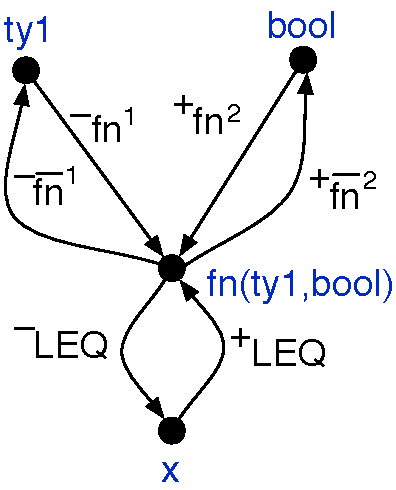
\includegraphics[width=0.19\textwidth]{graph/onecons}
    \label{fig:consgraph:first}
}
%
\subfigure[Constraint graph]{
    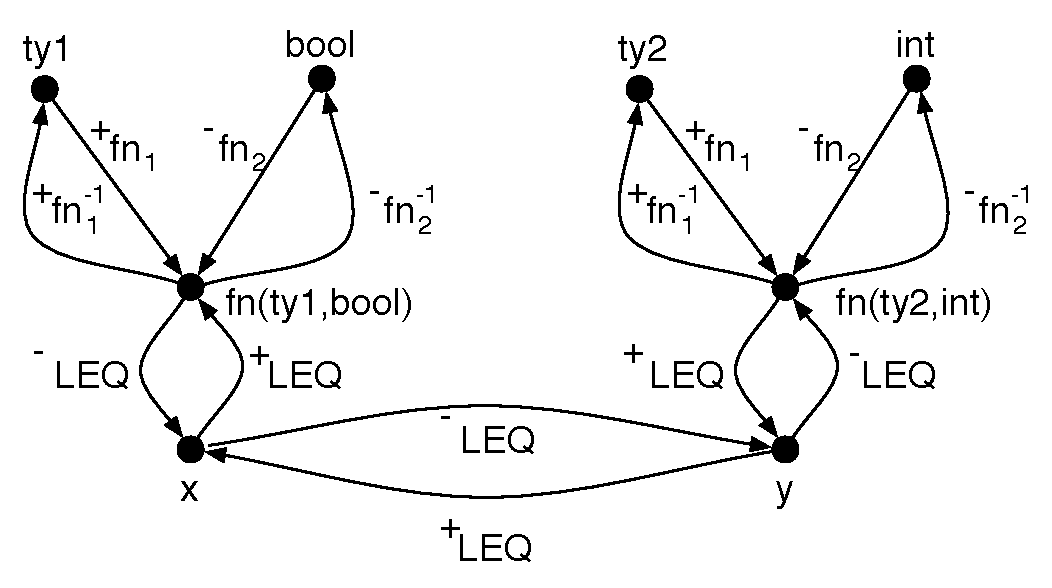
\includegraphics[width=0.4\textwidth]{graph/consexample}
    \label{fig:consgraph:second}
}
\end{center}
\caption{An example of constraint graph}
\label{fig:consgraph}
\end{figure*}

Constructor edges are labeled by the following information: the constructor,
position of the component, and the polarity (covariant, contravariant or
invariant). For instance, a label $\polarity{+}{\fn_1}$ means the first
component (which is covariant) of constructor $\fn$.
%
Decomposition edges are also added from the constructor to the components,
distinguished by a $(^{-1})$ in the graph.

To enable the flow from potentially contravariant variables, the LEQ edges,
representing $\leq$ relation, are duplicated in the reverse direction with
polarity $-$. For instance, there are two LEQ edges connecting $x$ and
$\fn(\cod{ty1},\cod{bool})$, with different polarity.

Some edges only exist when an assumption is true, like the third constraint
$\cod{ty2} \leq \cod{ty1} \proves y \leq x$. For assertions with hypotheses, we
construct the edges as discussed so far, and track the hypotheses on the edges.
Such information is used in the path finding process.

The transformed graph is shown in Figure~\ref{fig:consgraph:second}. The
systematic way of constructing a constraint graph from constrains is covered in
Section~\ref{sec:consgraph}.

More LEQ edges can be inferred in the constraint graph. For instance, following
the path from $\cod{bool}$ to $\cod{int}$ in Figure~\ref{fig:consgraph:second},
the constructor edges $\polarity{-}{\cod{fn}_2}$ and
$\polarity{-}{\cod{fn}_2^{-1}}$ cancels out. Similarly, we can infer another
LEQ edge from  $\cod{ty2}$ to $\cod{ty1}$. By the construction of graph, such
inferred LEQ edge must also hold if all the constraints in conclusion are true.
More generally, inferring all LEQ edge is a _all-pairs LEQ-path problem_, a
variance of _context-free-language reachability problems_ (CFL-reachability
problems). More details are discussed in Section~\ref{sec:leqedge}.

Given all pairs of nodes connected by LEQ edge (along the paths), the next step
is to check the inferred LEQ relation is satisfiable giving the hypothesis
along the edges. Since a constraint where either the LHS or RHS is a variable
is trivially satisfiable, there are two non-trivial LEQ pairs in
Figure~\ref{fig:consgraph:second}, namely $(\cod{bool, int})$ and $(\cod{ty2,
ty1})$. Notice that in order to infer these two LEQ relation, the hypothesis
along the path must hold too, which is $\cod{ty2}\leq \cod{y1}$ for both pairs.
Therefore, the satisfiability of the goal reduces to check the validity of two
assertions 
%
\[\cod{ty2}\leq \cod{y1}\proves \cod{bool}\leq \cod{int}\]
\[\cod{ty2}\leq \cod{y1}\proves \cod{ty2}\leq \cod{ty1}\]
, which is easy to tell that only the first assertion is invalid. Constraints
on the path from $\cod{bool}$ to $\cod{int}$ is a witness of the
unsatisfiability of the constraint set.

In general, checking the validity under hypothesis corresponds to check the LEQ
relation in the _hypothesis graph_, which we discuss in
Section~\ref{sec:hypograph}.

\subsection{Constructing constraint graph}
\label{sec:consgraph}

In this part, we describe the systematic way of transforming the constraints
into a constraint graph. Remind that the goal is an conjunction of assertion,
the algorithm works by adding assertions to graph one by one.

Given an assertion $C_1 \proves C_2$, hypothesis $C_1$ is saved in the
environment. Inequalities of $C_2$ are handled one by one.

Given an constraint $E_1 \leq E_2$ under environment $C$, we first transform
$E_1$ into conjunction normal form (CNF) and $E_2$ into disjunction normal form
(DNF): 
\[E_{11}\join E_{12} \join \dots \join E_{1n} \leq E_{21}\meet E_{22}
\meet \dots \meet E_{2m}\]

Since $\join$ and $\meet$ are standard least upper bound and greatest lower
bounds of the partial order, we can immediately break the constraint into
$n\times m$ _atomic constraints_: $E_{1i}\leq E_{2j}$, where $1\leq i\leq n
\land 1\leq j\leq m$.

To simplify the presentation, we assume that different elements have different
ids, and a unique node $N_{id}$ corresponds to element with $id$. There are
five different kinds of directed edges in the constraint graph, used in
Section~\ref{sec:leqedge}:

\begin{enumerate}
\item $LEQ$: an edge representing the partial ordering on source and sink

\item $\polarity{p}{cons_i}$: source is the $i$-th component of the sink. $p\in
\{+,-\}$ is the polarity of the component.

\item $\polarity{p}{cons_i^{-1}}$: the reverse of $cons$ edge

\item $join$: sink is a join element, and the source is one component

\item $meet$: sink is a meet element, and the source is one component

\end{enumerate}

For element $E$ with id $id$, graph is constructed in the following way:

\begin{itemize}
\item Variable $x$ or constant $c$: the graph contains node $N_{id}$. 

\item Constructor application $c(\polarity{p_1}{E_1}, \dots,
\polarity{p_2}{E_{\arity{c}}})$: for each $E_i$, $1\leq i \leq \arity{c}$,
the graph is constructed for $E_i$. Moreover, graph contains
$\polarity{p_i}{cons_i}$ edge from $E_i$'s node to $N_{id}$.  Also, create
$cons^{-1}(p_i,i)$ edge from $N_{id}$ to $E_i$'s node.

\item Projection $c^{-i}(E)$: construct graph for $E$. Also, create
$cons(p_i,i)$ edge from E's node to $N_{id}$ and create $cons^{-1}(p_i,i)$ edge
in the reverse direction.

\item Join $E_1\join E_2$: construct graph for both $E_1$ and $E_2$. Then,
create $\polarity{+}{LEQ}$ and $join$ edge from $E_1$ and $E_2$'s node to
$N_{id}$. Create $\polarity{-}{LEQ}$ in the reverse direction.

\item Meet $E_1\meet E_2$: construct graph for both $E_1$ and $E_2$. Then,
create $\polarity{+}{LEQ}$ edge from $N_{id}$ to $E_1$ and $E_2$'s node. Create
$meet$ and $\polarity{-}{LEQ}$ edge in the reverse direction.
\end{itemize}

Finally, for constraint $E_1\leq E_2$, construct graph for both $E_1$ and $E_2$. Then,
create $\polarity{+}{LEQ}$ edge from $E_1$'s node to $E_2$'s node, and
$\polarity{-}{LEQ}$ edge in the reverse direction.

\subsection{Inferring LEQ edges}
\label{sec:leqedge}

By construction, the inference of $\leq$ relation on the constraints is
transformed into the inference of LEQ edges in the constraint graph constructed
in Section~\ref{sec:consgraph}.

More specifically, the constraint graph can identify all provable $\leq$
ordering on elements by reducing the edges types according to the context-free
gramma shown in Figure~\ref{figure:cfg}. Finding all provable ``leq'' relation
in the graph is a _all-pairs LEQ-path problem_, a variance of
_context-free-language reachability problems_ (CFL-reachability problems),
which is used for a number of program-analysis applications~\cite{reps-graph}.
Both the reachability~\cite{melski-cflgraph} and shortest LEQ path
finding~\cite{barrett-cflpath} problems can be solved in polynomial time. We
adopt the dynamic programming approach~\cite{barrett-cflpath} to find the
shortest LEQ paths in this work. 

However, the CFG-reachability solution does not incorporate join and meet
edges. Hence, the graph may miss LEQ edges which can be inferred from the
constraints. For instance,  given constraints $a\meet b \leq c\land d\leq a
\land d\leq b$, by the rule $e\leq a\meet b \Iff e\leq a\land e\leq b$, we can
infer that $d\leq a\meet b \leq c$. 

To incorporate such inference into LEQ edge inference, whenever a LEQ edge
$LEQ(a,b)$ is processed, we check if this edge enables an join/meet inference
as follows. Let $JOIN(a)=\{n \bnf \exists. join(a,n) \}$ be the set of all join
elements where $a$ is a component. We check if all the components of such join
elements $J$ has a LEQ edge to $b$. If so, an LEQ edge is added from $J$ to
$b$. Meet elements are handled in a dual way.

\begin{figure}
\hfil
\begin{minipage}{2.3in}
\begin{align*}
\polarity{p}{LEQ} ::=\; & \polarity{p}{LEQ}\; \polarity{p}{LEQ}, p\in \{+,-\} \\
\polarity{p}{LEQ} ::=\; & \polarity{p}{c_i}\; \polarity{p}{LEQ}\; \polarity{p}{c_i^{-1}} \text{, where }  
    c\in \conset \land 1 \leq i\leq \arity{c} \land p\in \{+,-\}\\
\end{align*}
\end{minipage}
\caption{Context-free grammar of reduction}
\label{figure:cfg}
\end{figure}

\subsection{Hypothesis graph}
\label{sec:hypograph}

When algorithm in Section~\ref{sec:leqedge} infers a LEQ relation on two nodes,
all constraints constructing the corresponding edges automatically forms a
proof. However, the LEQ relation is valid only when all edges along the path
hold. That is, all the hypothesis along the path have to hold too.

Let $H_1, H_2, \dots, H_n$ be the hypothesis saved along the path from $a$ to
$b$, where $LEQ(a,b)$. 

Therefore, we can check the satisfiability of the subset of all constraints
along the path by checking the satisfiability of 
\[H_1 \land H_2 \land \dots \land H_n \proves a \leq b\]
, which is easy to test given the technique we discussed so far by noticing
that all the partial orders provable from the constraints in the hypothesis
must have a corresponding LEQ edge in the constraint graph constructed from the
hypothesis along, as described in Section~\label{sec:consgraph} and
Section~\ref{sec:leqedge}.

%The insight is consistent with ``A flow model FM is _secure_ if and only if
%execution of a sequence of operations cannot give rise to a flow that violates
%the relation $\rightarrow$''~\cite{denning-lattice}.

% First, for all the constraints in the right-hand-side, we
% first split the constraints into _atomic_ form according to the
% straightforward rules \DZ{only when the lattice is distributive}:
% 
% \[
% \G \proves l_1 \meet l_2 \meet \dots \meet l_m \leq r_1 \join r_2 \join \dots
% \join r_n
% \]
% 
% For constraints in this form, we generate nodes for each side, and
% add one _conditional edge_.
% 
% Static edges?
% 
% Back edges?
% 
% \DZ{No need} Conservative edge. When the right part constrains more
% than one variable, in general, satisfiability would be undecidable. As
% a common practice\DZ{true?}, we conservatively add edges from the
% union node to all variable components.
% 
\section{Ranking}
\label{sec:ranking}

The algorithm in Section~\ref{sec:graph} identifies unsatisfiable paths in the
constraint graph, which corresponds to a subset of unsatisfiable constraint
expressed by our constraint language. Reporting the information on a single
path already captures all information why the goal is unsatisfiable.

However, reporting all constraints along a path may still give too much
information that a programmer can digest. To alleviate such problem, we propose
to approaches to infer the likely cause of error: both a weakest and minimal
missing assumptions, and a most likely wrong subset of constraints that caused
the unsatisfiability based on maximum a posteriori principle.
 

\subsection{Inferring missing assumptions}
\label{sec:assumptions}

\subsection{Inferring likely wrong entities in program}

MAP model

\section{Evaluation}
\label{sec:evaluation}

\subsection{Extensibility}

\subsection{Ranking quality}

\section{Related Work}

\paragraph{Program analyses, constraints and graph} 

Modeling program analyses via constraint solving is not a new idea.
The most related work is set-based constraint program
analysis~\cite{aiken-setconstraint, aiken-typeinclusion}.  However,
these constraint languages do not model hypotheses, which is important
for some program analyses such as information-flow control.
 
Program slicing, shape analysis, and flow-insensitive points-to
analysis are amenable to graph-reachability~\cite{reps-graph}. Melski
and Reps~\cite{melski-cflgraph} show the interchangeability between
context-free-language reachability (CFG-reachability) and a subset of
set-based constraints. But only a small set of constraints---in fact,
a single variable---may appear on the right hand side of an partial
order. Moreover, no error diagnostic approach is proposed for the
graphs.

\paragraph{Error diagnoses for type inference
	    and information-flow control} 

Due to the unsatisfactory quality of error reports, a considerable
amount of work has been done on improving the error messages of both
ML-like languages and Jif.

Efforts on improving ML-like language type-error message can be
traced back to the early work of Wand~\cite{wand-errorfinding} and
of Johnson and Walz~\cite{johnson-popl86}. These two pieces of work
represent two directions in improving type-error messages: the former
traces _everything_ that contributes to the error, whereas the
latter attempts to infer the _most likely_ cause. We only discuss the
most related among them in this paper. More details can be found in
Heeren's summary~\cite{heeren:thesis}.

In the first direction, several efforts~\cite{choppella95,
haack:slicing, tip:slicing} improve the basic idea of
Wand~\cite{wand-errorfinding} in several ways. Despite the
attractiveness of feeding a full explanation to the programmer, the
reports are usually verbose and hard to follow.
\ACM{Can we cite anything for this claim of verbosity etc.? Right
now it is an unsupported assertion that doesn't sound very scientific.}

In the second direction, one approach is to alter the order of type
unification~\cite{lee:toplas, mcadam:unification}. However, since
error location may appear anywhere in the unification procedure, any
specific order fails in some circumstance. Some previous works tries
to advise the programmer how to fix the error.
McAdam~\cite{mcadam:thesis} suggests using morphisms along with
standard type inference to identify potential fixes for type errors.
Lerner et al.~\cite{lerner:pldi07} try to produce type-error messages
by trying changes to the AST until a program type-checks.  However,
both approaches are fairly specific to type inference. There is no
easy way of extending them for information-flow control analysis, for
instance.

For information-flow control, King et. al.~\cite{king:fse} propose to
generate a trace of information flow explaining the information-flow
violation in program. Despite the fact that this approach also
constructs a diagnosis from a dependency graph, only a subset of DLM
model is handled. In particular, hypotheses are not supported.
Moreover, as in type-error slicing, reporting a whole path can be
too verbose for the programmer.  Merlin~\cite{livshits:merlin} uses
probabilistic inference to automatically infer explicit information
flow specifications from program code; this is a different
application from our paper.\ACM{maybe we can say more about why Merlin
is relevant.}

\paragraph{Missing hypothesis inference}

The most related work on inferring likely missing hypotheses is the
recent work on error diagnosis using abductive
inference~\cite{dillig:pldi12}. This work computes small, relevant
queries presented to a user that capture exactly the information a
program analysis is missing to either discharge or validate the error.
It handles first-order logic, but there is no straightforward
way to encode our constraint language into first-order logic.
Also, our missing-hypothesis inference is more straightforward.
\ACM{Is it less powerful, though? Sounds a bit subjective.}

% Automatic instrumentation~\cite{king:esop10}
% Policy inference~\cite{chong:sp11, harris:ccs10}.
% Using statisctical
% analysis for bug finding is not new. Dawson Engler.

\bibliographystyle{abbrv}
\bibliography{constraint,../bibtex/pm-master}

\end{document}
